%
% frame.tex
%
% (c) 2019 Prof Dr Andreas Müller, Hochschule Rapeprswil
%
\section{Frame\label{section:frame}}
\rhead{Definition}
\index{Frame}%
Eine orthonormierte Basis eines Hilbertraumes ist sehr starr.
Es ist nicht möglich, auch nur einen einzigen Vektor ein kleines
Bisschen zu ändern, ohne die Eigenschaften, die zum Satz~\ref{satz:parseval}
geführt haben, zu zerstören.
Im Hinblick auf die numerische Behandlung von Signalen ist das
ein unerwünschter Zustand.
Rundungsfehler werden unvermeidlich dazu führen, dass solche strengen
Strukturen nur näherungsweise im Computer nachgebildet werden 
können.

Die Zerlegung eines Vektors $v$ in einer Orthonormalbasis enthält keine
Redundanz.
Geht einer der Koeffizienten $\hat{v}_k$ verloren, gibt es keine
Chance, den Vektor zu rekonstruieren.
Auch diese Situation ist unerwünscht, denn durch Rundungsfehler geht
mindestens ein Teil der Information in einem Koeffizienten verloren.
Wir suchen daher nach einer Verallgemeinerung des Basis-Begriffs, welche
auf kontrollierte Weise Redundanz in die Koeffizienten $\hat{v}_k$
bringt und damit eine robustere Konstruktion ermöglicht.

%
% Geometrisches Beispiel für ein Frame
%
\subsection{Ein geometrisches Beispiel
\label{subsection:hexagon}}
\begin{figure}
\centering
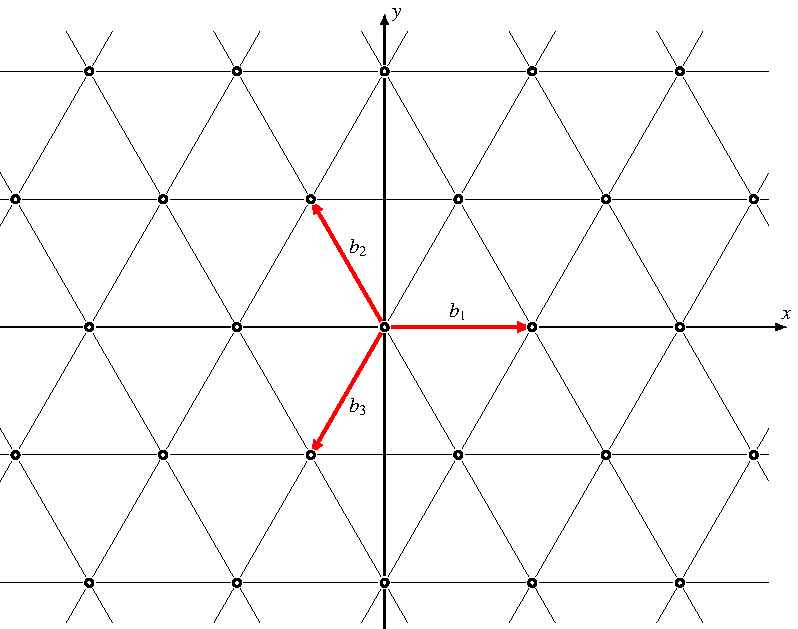
\includegraphics{chapters/1-geometrie/images/hexagon.pdf}
\caption{Sechseck-Gitter in der Ebene zum Frame $\{b_1,b_2,b_3\}$.
\label{geometrie:hexagon:image}}
\end{figure}
Wir suchen ein geeignetes Koordinatensystem, um ein Problem über
Bienenwaben in der Ebene zu lösen.
Dazu gehört das hexagonale Gitter in Abbildung~\ref{geometrie:hexagon:image}.
\index{hexagonal}%
\index{Bienenwaben}%
\index{Sechseck}%
Selbstverständlich kann dafür das übliche rechtwinklige Koordinatensystem
verwendet werden, aber die Ecken eines Sechsecks haben darin die nicht
sehr symmetrischen Koordinaten, die man in Abbildung~\ref{frame:hex:sechseck}
ablesen kann.
\begin{figure}
\centering
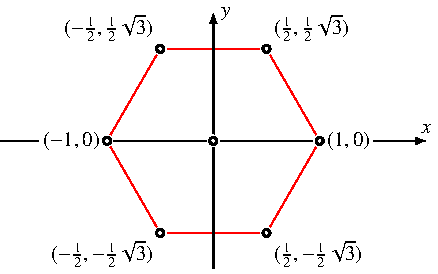
\includegraphics{chapters/1-geometrie/images/hexagon1.pdf}
\caption{Eckpunkte eines regelmässigen Sechsecks sollen mit der
Basis \eqref{frame:hex:basis} analysiert werden
\label{frame:hex:sechseck}}
\end{figure}
(Siehe auch Abbildung~\ref{geometrie:hexagon:image}).
Eine bessere Variante ist das Koordinatensystem auf der Basis der beiden
Basisvektoren (in kartesischen Koordinaten)
\begin{equation}
\begin{aligned}
b_1 = \begin{pmatrix} 1\\0\end{pmatrix}
\qquad
\text{und}
\qquad
b_2 = \begin{pmatrix} -\frac12\\\frac12\sqrt{3}\end{pmatrix}.
\end{aligned}
\label{frame:hex:basis}
\end{equation}
In diesem Koordinatensystem haben die Ecken des Sechsecks die Koordinaten
wie in Abbildung~\ref{frame:hex:basisanalyse}
\begin{figure}
\centering
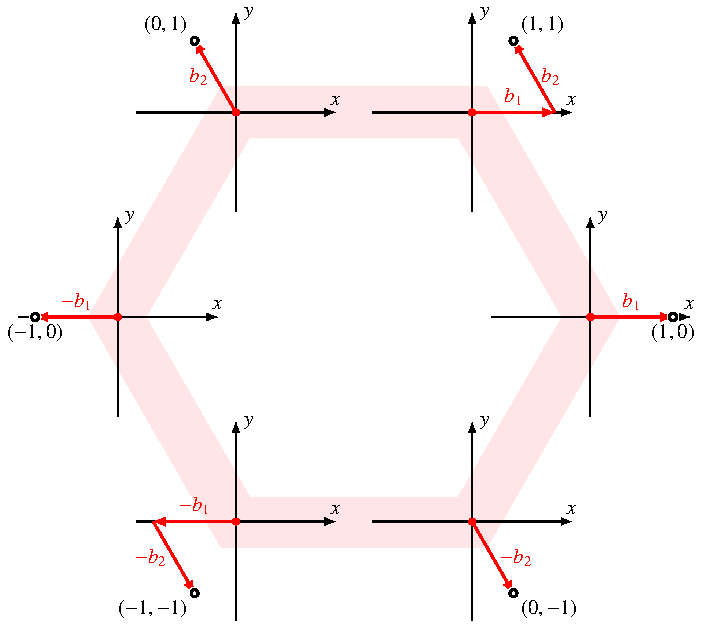
\includegraphics{chapters/1-geometrie/images/hexagon2.pdf}
\caption{Darstellung der Ecken des Sechsecks in der
Basis~\eqref{frame:hex:basis}
\label{frame:hex:basisanalyse}}
\end{figure}
Dies bereits viel symmetrischer aus.
Trotzdem ist auch dies noch nicht ganz zufriedenstellend. 
Zum Beispiel sind die Ecken links oben und rechts unten direkt durch den
Basisvektor $b_2$ darstellbar, die Ecken rechts oben und links unten
dagegen nur durch eine Linearkombination.
Wir könnten natürlich auch die linke untere Ecke als Basisvektor nehmen,
dann würde eiinfach die linke obere Ecke speziell.
In dieser Situation lässt es sich also mit einer Basis gar nicht erreichen,
dass alle Eckpunkte sich auf einfache Art darstellen lassen.

Verzichten wir jedoch darauf, dass die Vektoren linear unabhängig sein müssen,
können wir als ``Basis'' die drei Vektoren (in kartesischen Koordinaten)
\begin{equation}
\begin{aligned}
b_1
&=
\begin{pmatrix}1\\0\end{pmatrix},
&
b_2
&=
\begin{pmatrix}-\frac12\\\frac12\sqrt{3}\end{pmatrix}
&&\text{und}
&
b_3
&=
\begin{pmatrix}-\frac12\\-\frac12\sqrt{3}\end{pmatrix}
\end{aligned}
\label{hexagonbasis}
\end{equation}
verwenden.
Die drei Vektoren haben alle die Länge $1$, aber sie sind nicht
orthogonal, sondern haben die Skalarprodukte
\[
\langle b_j,b_k\rangle
=
\begin{cases}
-\frac12&\qquad j\ne k\\
1&\qquad j=k.
\end{cases}
\]
Zu jedem Vektor $v\in\mathbb R^2$ können wir wieder eie Koeffizienten
$\hat{v}_k=\langle v,b_k\rangle$ berechnen und damit die Linearkombination
\[
v' = \sum_{k=1}^3 \hat{v}_k\,b_k
\]
bilden,
doch es ist $v\ne v'$.
Wir führen dies durch für die Basisvektoren:
\begin{align*}
b_1'
&=
b_1 - \frac12 b_2 - \frac 12 b_3
=
\frac32b_1
\\
b_2'
&=
-\frac12 b_1 + b_2 -\frac12 b_3
=
\frac32b_2
\\
b_3'
&=
-\frac12b_1-\frac12 b_2 + b_3
=
\frac32b_3
\end{align*}
Daraus lässt sich durch Linearkombination die Synthese auch für jeden
anderen Vektor durchführen.
Sie liefert nicht den ursprünglichen Vektor, sondern
\begin{equation}
\sum_{k=1}^3 \hat{v}_k b_k = \frac32\,v
\label{geometrie:32beispiel}
\end{equation}
zurück, das $\frac32$-fache davon.
Dies ist bereits ein Ausdruck der Tatsache, dass die Information in den
Koeffizienten $\hat{v}_k$ redundant ist.
Andererseits zeigt dies auch, dass alle Richtungen gleichermassen
verzerrt werden.

Die Vektoren~\eqref{hexagonbasis}
sind natürlich nicht mehr linear unabhängig, Vektoren
der Ebene können also auf verschieden Art linear aus den $b_k$ kombiniert
werden.
Da $b_1+b_2+b_3=0$ ist, kann man zu den Koeffizienten $\hat{v}_k$
eine beliebige Zahl $\alpha$ hinzuaddieren und erhält
\[
\sum_{k=1}^3 (\hat{v}_k+\alpha)\, b_k
=
\sum_{k=1}^3 \hat{v}_k\,b_k
+\alpha
\underbrace{ \sum_{k=1}^3 b_k}_{\displaystyle=0}
=
\sum_{k=1}^3 \hat{v}_k\,b_k
=
\frac32 v.
\]
Die modifizierten Koeffizienten ergeben also das gleichen synthetisierten
Vektor $\frac32 v$.

Für die Norm des synthetisierten Vektors gilt natürlich
\[
\|v'\|^2
=
\frac94\|v\|^2
=
\sum_{k=1}^3 \hat{v}_k^2 
-
\frac12\sum_{k\ne l} \hat{v}_k\hat{v}_l.
\]

Was zeichnet die Koeffizienten $\hat{v}_k$ gegenüber den modifizierten
Koeffiziente $v_k$ aus?
In Abbildung~\ref{3dbasisbild} sind die Koeffizienten $\hat{v}_k$ als
dreidimensionaler Vektor $v'$ dargestellt.
Punkte in der Ebene werden durch die Analyse mit Hilfe der Vektoren $b_k$
auf Vektoren in der hellblau hervorgehobenen Ebene abgebildet.
Die alternativen Linearkombinationen entstehen, indem man zu $v$
ein Vielfaches des grünen Normalenvektors $n$ hinzuaddiert.
Die gelb gezeichneten Punkte $w$ bilden eine Gerade senkrecht
auf der hellblauen Ebene.
Alle Punkte auf dieser Geraden führen auf die gleiche
Linearkombination $\frac32v$.
Die mit Hilfe der Skalarprodukte gefundene Linearkombination
$\hat{v}_k=\langle v,b_k\rangle$ hat daher die Eigenschaft, 
$v'$ unter all den Punkte auf der Geraden die kürzeste Länge hat.
Oder: die Koeffizienten $\hat{v}_k$ zeichnen sich unter allen
Koeffizienten $v_k$ mit der gleichen Linearkombination dadurch aus, 
dass
\begin{equation}
\|v'\|^2
=
\sum_{k=1}^n |\hat{v}_k|^2
\le
\sum_{k=1}^n |v_k|^2
\qquad
\text{für Koeffizienten $v_k$ mit}
\quad
\sum_{k=1}^3 \hat{v}_kb_k
=
\sum_{k=1}^3 v_kb_k
\label{hexagonbasiseigenschaft}
\end{equation}
ist.
Die durch $\hat{v}_k$ gefundenen Koeffizienten zeichnen sich durch
die minimale ``Koeffizientenenergie'' aus.

Im Falle einer Orthonormalbasis konnte man dank der Plancherel-Formel
die Norm eines Vektors mit Hilfe der Quadratsumme der Koeffizienten
berechnen.
Die Eigenschaft \eqref{hexagonbasiseigenschaft} kann also als erweiterte
Form der Plancherel-Formel angesehen werden.

\begin{figure}
\centering
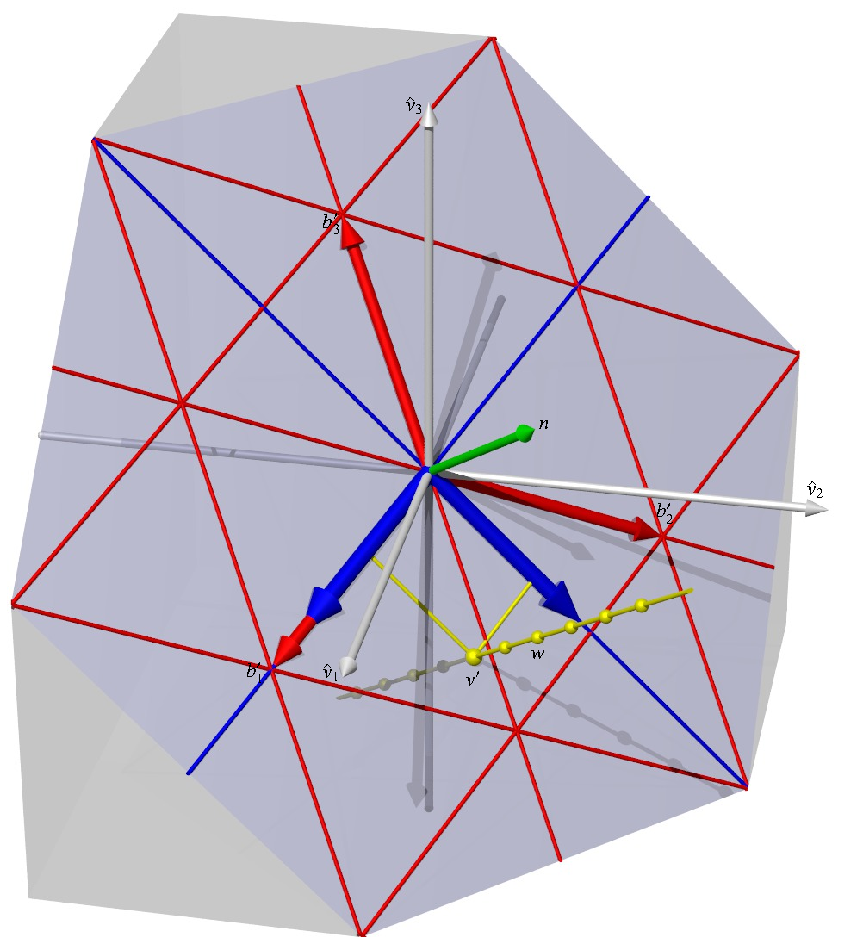
\includegraphics{chapters/1-geometrie/images/tri.pdf}
\caption{Darstellung der Koeffizienten $\hat{v}_k$ bezüglich Vektoren $b_i$
aus \eqref{hexagonbasis}.
Die drei Vektoren $b_i$ haben als $\hat{v}_k$-Koeffizienten-Vektoren
die Vektoren $b_i'$.
Die $x$- und $y$-Achsrichtung werden auf die beiden blauen Vektoren
abgebildet.
Ein Vektor $v$ wird auf den Vektor $v'$ mit den Komponenten
$\hat{v}_k$ abgebildet.
Die Darstellung eines Vektors als Linearkombination der $b_i$ ist
jedoch nicht eindeutig.
Ändert man die Koeffizienten um den gleichen Wert, was gleichbedeutend damit
ist, dass man dem Vektor $v'$ ein Vielfaches von $n$ hinzufügt, entsteht
bei der Synthese $\sum \hat{v}_k b_k$ der gleiche Punkt.
Alle gelben Punkte $w$ sind daher Koeffizienten, die den gleichen Punkt $v$
ergeben, wenn man damit die Vektoren $b_i$ linear kombiniert.
\label{3dbasisbild}}
\end{figure}

%
% Definition eines Frames
%
\subsection{Definition eines Frames}
Nach dem motivierenden Beispiel im vorangegangenen Abschnitt sind wir nun
bereit, eine allgemeine Definition aufzubauen.
Wir wollen also weiterhin die Vektoren eines Vektorraums $V$ mit Hilfe
einer Menge von Vektoren $\{e_k\,|\,1\le k\le n\}$ linear kombinieren,
verlangen aber nicht mehr, dass die Vektoren $e_k$ linear unabhängig sind.
Dies bedeutet natürlich, dass die Darstellung eines Vektors $v\in V$
nicht mehr eindeutig sein wird.

Nicht jede Menge von Vektoren $\{e_k\,|\,1\le k\le n\}$ ist geeignet.
Es muss ja immer noch jeder Vektor dargestellt werden können, das
Erzeugnis $U := \langle e_k\,|\,1\le k\le n\rangle$
der Vektoren muss also der ganze Vektorraum sein:
\[
U
=
V.
\]
Wäre das Erzeugnis nur ein echter Unterraum $U\subset V$, dann gäbe es
einen Vektor $b\in V$, der senkrecht steht auf allen $b\perp U$.
Wir fordern daher, dass es keinen Vektor gibt, der auf allen Vektoren $e_k$
senkrecht steht.
Nach Definition~\ref{geometrie:erzeugendensystem} bilden die
Vektoren $e_k$ ein Erzeugendensystem.

Damit die Berechnung effizient bleibt, möchten wir weiterhin nur mit den
Koeffizienten $\hat{v}_k = \langle v,e_k\rangle$ arbeiten.
Für eine Orthonormalbasis hat die Plancherel-Formel gezeigt, dass
\[
\sum_{k=1}^n |\hat{v}_k|^2 = \|v\|^2.
\]
In der aktuellen Situation können wir nicht mehr erwarten, dass dies 
weiterhin funktioniert.
Wir müssen aber mindestens verlangen, dass die Transformation
\[
\mathcal{T}
\colon
V\to \mathbb R^n
:
v\mapsto \hat{v}_k
\]
stetig ist, dass sich also kleine Änderungen von $v$ ebenfalls
kleinen Änderungen des Vektors der $\hat{v}_k$ auswirken.
Es muss also eine Konstante $B$ geben, so dass
\[
\sum_{k=1}^n |\hat{v}_k|^2
=
\sum_{k=1}^n |\langle v,e_k\rangle|^2
\le
B \|v\|^2.
\]

Wir müssen aber auch sicherstellen, dass die Rekonstruktion des Vektors $v$
auf stetige Art von den Koeffizienten $\hat{v}_k$ abhängt. 
Eine kleine Änderung der Koeffizienten darf sich nur in beschränkten Änderungen
im rekonstruierten Vektor $v$ auswirken.
Es muss also eine Konstante $A$ geben, so dass
\[
\sum_{k=1}^n |\hat{v}_k|^2
=
\sum_{k=1}^n |\langle v,e_k\rangle|^2
\ge
A \| v \|^2
\]
gilt.

Damit haben wir alle Elemente zusammen für die folgende Definition,
die auch für unendlichdimensionale Hilberträume funktioniert.

\begin{definition}
\label{definition:frame}
Eine Teilmenge $\{ e_k\,|\, k\in K\}\subset V$ heisst ein {\em Frame},
\index{Frame}%
wenn es zwei positive Konstanten $A>0$ und $B>0$ gibt, so dass
\[
A\|v\|^2 \le \sum_{k\in K} |\langle v, e_k\rangle|^2 \le B \| v\|^2
\]
gilt für jeden Vektor $v\in V$.
Die Konstanten $A$ und $B$ heissen die {\em Framekonstanten} des Frames.
\index{Framekonstante}%
Das Frame heisst {\em straff}, wenn $A=B$ ist.
\index{straff}%
\end{definition}

\begin{beispiel}
Das Beispiel von Abschnitt~\ref{subsection:hexagon} ist ein Frame.
Die Formel \eqref{geometrie:32beispiel} zeigt, dass die Framekonstanten
des Frames $A=B=\frac32$ ist.
Das Frame ist also sogar straff.
\end{beispiel}

In der Definition wird nicht erwähnt, dass die Vektoren des Frames den
ganzen Raum aufspannen müssen.
Diese Eigenschaft folgt jedoch direkt aus der Definition eines Frames,
wie der folgende Satz zeigt.

\begin{satz}
\label{geometrie:frame:erzeugt}
Ist $\mathcal{B}=\{ e_k\,|\, k\in K\}$ ein Frame des Hilbertraumes $V$
mit Framekonstanten $A$ und $B$, dann gibt es keinen Vektor $v\in V$,
der auf allen Vektoren $e_k$ senkrecht steht.
\end{satz}

\begin{proof}[Beweis]
Nehmen wir an, es gäbe einen Vektor $v\in V$ mit $\langle v,e_k\rangle=0$
für alle $k\in K$.
Dann folgt aus den Frame-Ungleichungen
\[
\| v \|^2 \le \frac1{A} \sum_{k\in K} |\langle v,e_k\rangle|^2 = 0
\qquad\Rightarrow\qquad
v=0.
\]
Der Nullvektor ist also der einzige Vektor, der auf allen Framevektoren
senkrecht steht.
\end{proof}

Eine orthonormierte Basis war die bevorzugte Wahl für eine Basis, weil
sich damit die Transformation $\mathcal{T}$ besonders leicht invertieren
lässt.
Der Satz~\ref{satz:parseval} hat gezeigt, dass die Transformation %$\mathcal{T}$
eine Isometrie ist, insbesondere gilt
\[
\|v\|^2
=
\sum_{k\in K} |\hat{v}_k|^2
=
\sum_{k\in K} |\langle v,e_k\rangle|^2.
\]
Dies bedeutet, dass eine orthonormierte Basis ein straffes Frame mit
Framekonstanten $A=B=1$ ist.
Umgekehrt drängt sich die Frage auf, ob straffe Frames oder spezielle
Werte der Frame-Konstanten eine besondere Bedeutung für die Invertierbarkeit
haben.

\begin{figure}
\centering
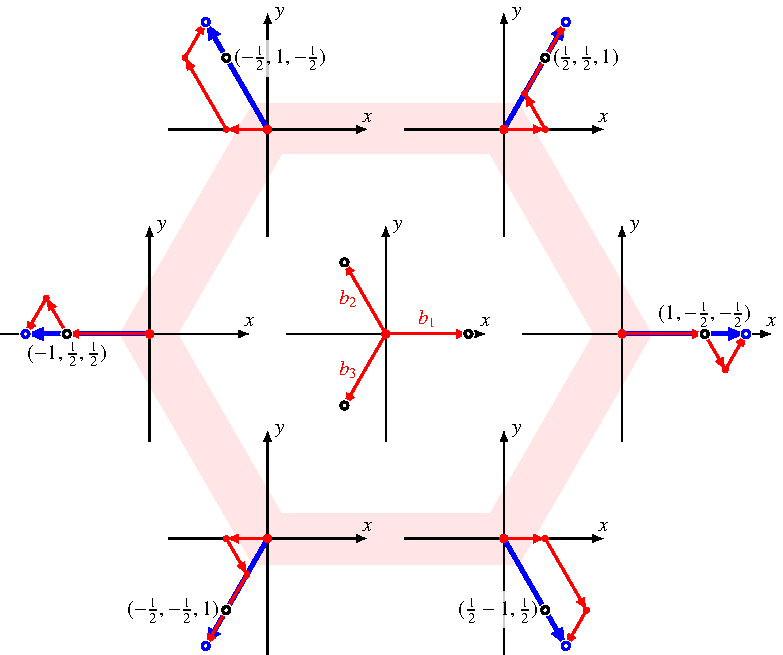
\includegraphics{chapters/1-geometrie/images/hexagon3.pdf}
\caption{Rekonstruktion bei einem straffen Frame.
Das Frame bestehend aus den Vektoren $\{b_1,b_2,b_3\}$ ist straff
mit der Framekonstanten $A=\frac32$.
Die mit den Skalarprodukten gewichtete Linearkombination der
Framevektoren liefert nicht den ursprünglichen Vektor zurück, sondern
einen Vektor, der mit der Framekonstanten multipliziert wird.
Gezeigt wird dies für die sechs Ecken des Hexagons.
Die Skalarprodukte mit den Framevektoren, die Framekoordinaten, sind
als Zahlentripel bei jedem Punkt angegeben.
Die roten Vektorpfade stellen die Linearkombination dar, die blauen
Vektoren die Summe.
\label{geometrie:hexagon:rekonstruktion}}
\end{figure}

%
% Frames in R^n
%
\subsection{Frames in $\mathbb R^n$
\label{subsetion:skript:frames:framesinrn}}
Wir betrachten jetzt den Spezialfall $H=\mathbb{R}^n$ mit dem
Standardskalarprodukt.
Jeder endlichdimensionale Hilbertraum lässt sich durch Wahl einer
Orthonormalbasis in dieser Form beschreiben.
Das Beispiel von Abschnitt~\ref{subsection:hexagon} ist ein Beispiel für
den Fall $\mathbb R^2$.

Ein Frame in $\mathbb R^n$ ist nach Definition~\ref{definition:frame}
eine Menge 
\[
\mathcal{B}
=
\{b_1,\dots,b_m\}
\subset
\mathbb R^n
\]
von Vektoren in $\mathbb R^n$ mit zwei positiven Konstanten $A$ und $B$
derart, dass
\[
A\|v\|^2
\le
\sum_{k=1}^m |\langle v,b_k\rangle|^2
\le
B\|v\|^2
\]
gilt für jeden Vektor $v\in\mathbb R^n$.
Da alle beteiligten Vektorräume endlichdimensional sind, können
die Abbildungen als Matrizen beschrieben werden.
Ziel dieses Abschnitts ist, neben einer Matrizenbeschreibung
der Frame-Abbildung $\mathcal{T}$ auch eine Formel für die
Umkehrabbildung zu finden.

In einem endlichdimensionalen Raum ist die Frame-Bedingung $A>0$ 
nach Satz~\ref{geometrie:frame:erzeugt}
gleichbedeutend damit, dass die Frame-Vektoren den ganzen Raum erzeugen.

\subsubsection{Der Frame-Operator}
\index{Frame-Operator}
Der Frame-Operator berechnet die Analysekoeffizienten
$\hat{v}_k=\langle v,b_k\rangle$ eines Signals
$v\in \mathbb R^n$ bezüglich des Frames $\mathcal{B}$:
\[
\mathcal{T}\colon \mathbb R^n \to \mathbb R^m
:
v \mapsto
\begin{pmatrix}
\hat{v}_1\\\hat{v}_2\\\vdots\\\hat{v}_m
\end{pmatrix}
=
(\hat{v}_k=\langle v,b_k\rangle)_{1\le k\le m}.
\]
Zur Berechnung der Skalarprodukte kann man das Matrizenproukt
\[
\langle v,b_k\rangle
=
b_k^t v
\]
verwenden.
Die Zeilenvektoren $b_k^t$ kann man zeilenweise in einer grossen Matrix $T$
\[
T 
=
\begin{pmatrix}
\dots&b_1^t &\dots\\
\dots&b_2^t &\dots\\
     &\vdots&     \\
\dots&b_m^t &\dots
\end{pmatrix}
\]
zusammenführen.
Das Matrixprodukt $Tv$ liefert dann genau das Resultat des Frame-Operators
\[
\mathcal{T} v
=
\begin{pmatrix}
\langle v, b_1\rangle\\
\langle v, b_2\rangle\\
\vdots\\
\langle v, b_m\rangle\\
\end{pmatrix}
=
\begin{pmatrix}
b_1^tv\\
b_2^tv\\
\vdots\\
b_m^tv\\
\end{pmatrix}
=
\begin{pmatrix}
\dots&b_1^t &\dots\\
\dots&b_2^t &\dots\\
     &\vdots&     \\
\dots&b_m^t &\dots
\end{pmatrix}
v
=
Tv.
\]
Die Matrix $T$ ist die Matrix des Frame-Operator $\mathcal T$ bezüglich der
Standardbasis von $\mathbb R^n$.

\begin{beispiel}
Im Beispiel von Abschnitt~\ref{subsection:hexagon} besteht das Frame
aus den Vektoren
\[
\mathcal{B}
=
\biggl\{
\begin{pmatrix}1\\[2pt] 0\end{pmatrix},
\begin{pmatrix}-\frac12\\[2pt] \frac{\sqrt{3}}2\end{pmatrix},
\begin{pmatrix}-\frac12\\[2pt] -\frac{\sqrt{3}}2\end{pmatrix}
\biggr\}.
\]
Der zugehörige Frameoperator $\mathcal{T}$ hat daher die Matrix
\begin{equation}
T
=
\begin{pmatrix}
1&0\\[2pt]
-\frac12&\frac{\sqrt{3}}2\\[2pt]
-\frac12&-\frac{\sqrt{3}}2
\end{pmatrix}.
\label{beispielTmatrix}
\end{equation}
\end{beispiel}

